\chapter{\textbf{Entorno empresarial}}

\thispagestyle{empty}

\section{Descripción}

Turpial Development es una empresa mediana, con 4 años en el mercado que está enfocada en el desarrollo de sistemas y aplicaciones Web y Móviles. Fundada e integrada por jóvenes venezolanos y ofrece soluciones que cumplen con altos estándares de usabilidad, diseño y funcionalidad.

\section{Misión}

La empresa tiene como misión “prestar servicios y consultoría en diseño y desarrollo de soluciones web, a la medida del cliente, caracterizadas por una alta calidad, excelente soporte y experiencia de usuario”. (Manual para desarrolladores, 2016)


\section{Visión}

Su visión es “servir de plataforma para el desarrollo y éxito de nuevos emprendimientos en el área web”. (Manual para desarrolladores, 2016)

\section{Estructura}

\begin{description}
    \item \textbf{Dirección de Operaciones}
    \item \textbf{Dirección de Proyectos}
    \item \textbf{Dirección de Desarrollo}
    \item \textbf{Dirección de Diseño}
    \item \textbf{Dirección de Mercadeo}
\end{description}

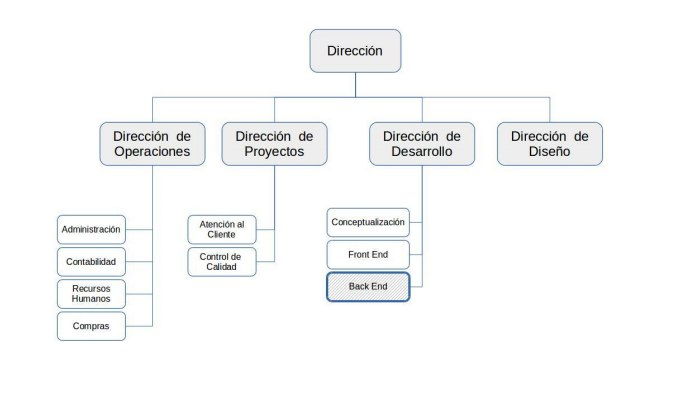
\includegraphics{Estructura_Turpial.png}

El desarrollo de la pasantía fue llevado a cabo en la Dirección de Desarrollo de la empresa. El pasante fue asignado al departamento de \textit{Backend} bajo el cargo de Pasante, para cumplir tareas tales como: levantar requerimientos, diseñar y desarrollar las funcionalidades de la solución propuesta para el sistema. 



